\section{Approach}
\label{sec:approach}

% MDPs
Before we describe our approach for generating options, we briefly review Markov
Decision Processes (MDPs) and options framework. An MDP $\tuple{
    \states,\actions,\rewards }$ is a standard representation for a RL problem,
where $\states$ is the set of states in the world, $\actions$ is the set of
actions that take the agent from one state to another with some transition
probability, and $rewards$ is the set of rewards obtained when moving from one
state to another. The objective is to find a decision procedure or policy $\pi$
that maximises the return, or the rewards accumulated in the long run. 

% Options
An option $\option$ is described by an initiation set $\initset \subset
\states$, a policy $\pi$, and a terminating condition $\beta$. An agent can
exercise an option in any state $s \in \initset$, following which, it will
follow the policy $\pi$ described by the option, until the terminating condition
$\beta(s)$ is satisfied. The terminating condition $\beta$ can be stochastic as
well. 

% Example

\begin{figure}[h]
    \center
    \documentclass{article}
\usepackage{tikz}
\usetikzlibrary{external}
\usetikzlibrary{arrows}
%\tikzexternalize % activate!

\begin{document}
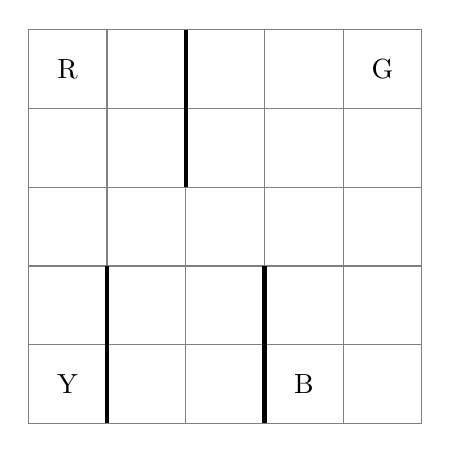
\begin{tikzpicture}
    % Grid
    \draw[step=1,color=gray] (0,0) grid (5,5);
    
    % Walls
    \draw[line width=1.5pt] (2,5) -- (2,3);
    \draw[line width=1.5pt] (1,0) -- (1,2);
    \draw[line width=1.5pt] (3,0) -- (3,2);

    % Pads
    \draw (0.5,4.5) node {R};
    \draw (0.5,0.5) node {Y};
    \draw (3.5,0.5) node {B};
    \draw (4.5,4.5) node {G};
\end{tikzpicture}
\end{document}

    \caption{The Taxi Domain}
    \label{fig:taxi-domain}
\end{figure}

To make the discussion more tangible, let us look at an example, the Taxi
domain, shown in \autoref{fig:taxi-domain}. The agent is a taxi navigating in
this road-map. It must pick up a passenger at one of the 4 pads, A, B, C or D.
Subsequently, it must carry the passenger to a destination, which is also one of
the above four pads. The states of the taxi would then be the location of the
passenger (in one of the four pads, or within the taxi), the destination of the
passenger, and location of the taxi in the map. The actions the taxi can perform
are moving up, down, left or right in the map, as well as pick up a passenger or
drop him at the destination.  Typical options for such a domain would be an
option that can be started anywhere, and has a policy that takes the taxi to the
one of the pads in the shortest possible manner. Such an option is generic, and
does not depend on where the passenger or destination are. The RL agent must
then learn to choose the right option when picking up the passenger.

\begin{figure}[h]
    \center
    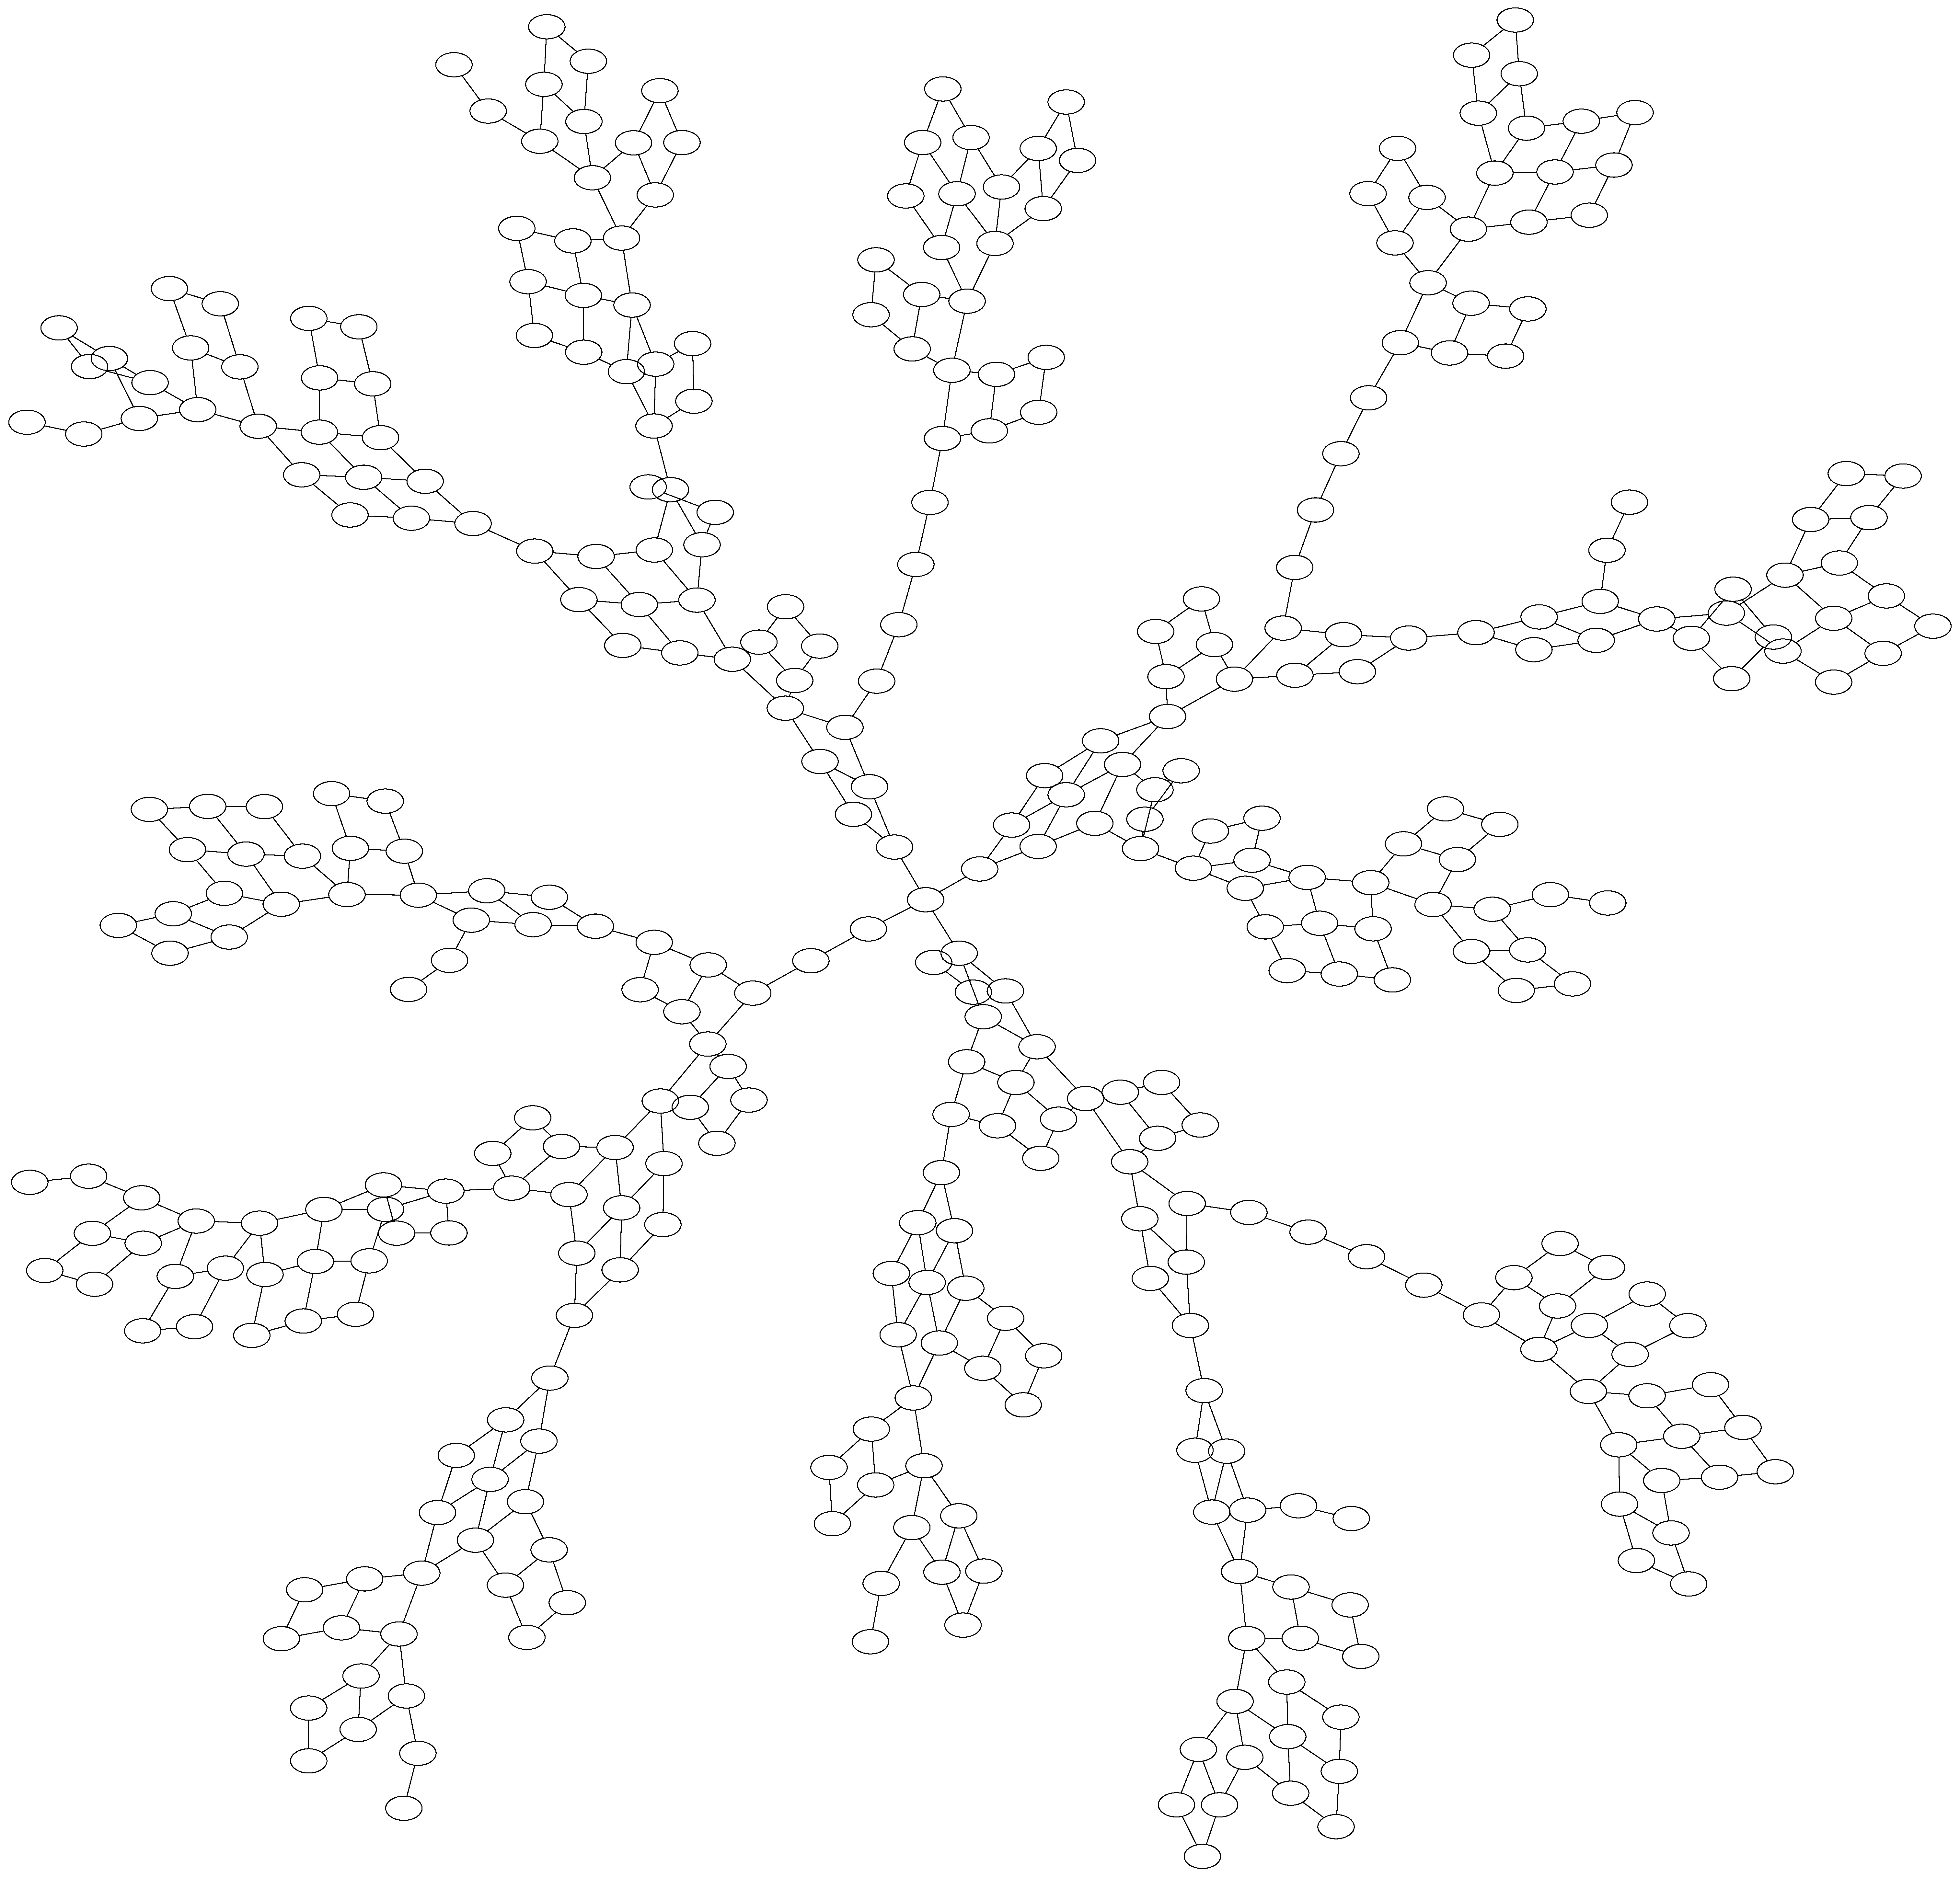
\includegraphics[width=3in]{figures/taxi1}
    \caption{State Space Graph for the Taxi Domain}
    \label{fig:taxi-graph}
\end{figure}

% Graph-based
It is easy to construct a graph $\graph$ out of the state-space described by an
MDP. The states $\states$ become the nodes of the graph, and $\actions$ become
the edges, with the transition probabilites serving as the weights. The edges
are also attributed with the rewards described by $\rewards$. Options can be
viewed to be paths along the graph. The Taxi domain just defined translates to
a graph shown in \autoref{fig:taxi-graph}.

% Constructing Options 
We construct an option `short-circuiting' two states using a policy constructed
from the shortest path on this graph. For every state $x$, we select a state to
be short-circuited $y$ with using a multinomial distribution with weight
proportional to the distance between them in the state space, i.e. $w(x,y)
    \propto d(x,y)^{-r}$. 

Another example of constructing an option on this graph would be to define a
policy that takes any state to a particular one along the shortest path. This is
the approach adopted by Simsek and Barto in \cite{Simsek}, where local maxima of
the betweenness scores are used to identify bottlenecks, and options defined to
reach these bottlenecks optimally from any state.

% Describe Macro-Q and Intra-Option-Q
Several learning algorithms have been proposed for agents using options
\cite{SuttonPrecupSingh1998,BartoMahadevan}. A simple such method is Macro
Q-learning, a generalisation of the Q-learning methods. The MacroQ algorithm
updates the value function only after completion of the option. If the option
$o$ was initiated in the state $s$, and continue for $k$ steps before
terminating in $s'$, the corresponding back-up will be,

\begin{IEEEeqnarray*}{rCl}
    Q(s,o) &=& Q(s,o) + \alpha [ r + \gamma^{k} \max_{o' \in \options_{s'} \cup \actions_{s'}} Q(s',o') - Q(s,o) ].
\end{IEEEeqnarray*}

Another method, Intra-option Q-learning, exploits the experience gathered during
the trajectory, instead of only at the end of it. In this approach, every step
from $s$ to $s'$ using $a \in \actions$ is used to back up the value function of
every option $o \in \options$ which can be used in $s$, and whose policy has a
non-zero probability of using the action $a$ using the following update,

\begin{IEEEeqnarray*}{rCl}
    Q(s,o) &=& Q(s,o) + \alpha [ r + \gamma Q(s',o) - Q(s,o) ].
\end{IEEEeqnarray*}
\noindent
The value-function for every action along the trajectory is also updated, using
the usual Q-learning backups.

% \begin{IEEEeqnarray*}{rCl}
%     x &=& y \\
%       &=& z \\
% \end{IEEEeqnarray*}

% \begin{figure}[s]
%     \centering
%     \includegraphics[width=5in]{filename}
%     \caption{ }
%     \label{fig:high-variance-rtt}
% \end{figure}
